% =============================================================================
% Master's Thesis -- Nova SBE -- Business Analytics
% Cold-Start Preference Alignment of LLMs: a Comparative Study
% =============================================================================
%
% Build:
%   latexmk -pdf main.tex          (recommended)
%   or:  pdflatex main && biber main && pdflatex main && pdflatex main
%
% Note: this revision switches the bibliography to Chicago Author-Date
% (biblatex-chicago, authordate style), as recommended by the Nova SBE
% Library for work projects. The cover page is the official Nova SBE WP
% template with the abstract and keywords on the same page, plus the
% mandatory FCT / LISBOA2030 funding acknowledgement.
% =============================================================================

\documentclass[12pt,a4paper]{article}

% ------ Encoding / fonts ----------------------------------------------------
\usepackage[T1]{fontenc}
\usepackage[utf8]{inputenc}
\usepackage{lmodern}
\usepackage{microtype}
\usepackage[english]{babel}

% ------ Page layout ---------------------------------------------------------
\usepackage[a4paper,margin=2.5cm]{geometry}
\usepackage{setspace}
\onehalfspacing
\usepackage{parskip}      % space between paragraphs, no indent

% ------ Math & symbols ------------------------------------------------------
\usepackage{amsmath,amssymb,amsthm,mathtools}
\usepackage{siunitx}
\sisetup{detect-all,group-separator={,},group-minimum-digits=4}

% ------ Graphics, tables, floats --------------------------------------------
\usepackage{graphicx}
\graphicspath{{figures/}}
\usepackage{booktabs}
\usepackage{tabularx}
\usepackage{multirow}
\usepackage{caption}
\captionsetup{font=small,labelfont=bf}
\usepackage{placeins}

% ------ Code / pseudocode ---------------------------------------------------
\usepackage{listings}
\lstset{
  basicstyle=\ttfamily\small,
  breaklines=true,
  frame=single,
  showstringspaces=false,
}

% ------ Bibliography (Chicago Author-Date via biblatex-chicago) -------------
% Style produces:
%   In-text:      (Chiang et al. 2024)        -- no comma
%   Bib entry:    Chiang, Wei-Lin, Lianmin Zheng, ... 2024. "Title." Source.
% maxbibnames=7 forces "first 7 + et al." in the reference list, matching
% Nova SBE's instruction for articles with more than 10 authors.
\usepackage{csquotes}
\usepackage[
  authordate,            % Chicago Author-Date
  backend=biber,
  natbib=true,           % keep \citep / \citet from old source
  maxcitenames=2,        % "Author1 and Author2" before "Author1 et al."
  maxbibnames=7,         % cut to first 7 + et al. in bibliography
  minbibnames=7,         % when cutting, keep exactly 7
  giveninits=false,
  uniquename=false,
  uniquelist=false,
]{biblatex-chicago}
\addbibresource{references.bib}

% ------ Cross-references (load hyperref LAST, cleveref AFTER) ---------------
\usepackage[hidelinks]{hyperref}
\usepackage[noabbrev,capitalize]{cleveref}

% ------ Convenience macros --------------------------------------------------
\usepackage{xcolor}
\long\def\todo#1{{\color{red}\bfseries [TODO: #1]}}

% =============================================================================
\begin{document}

% =============================================================================
% Official Nova SBE WP cover page (Template_WP_Cover_Page_Abstract_NovaSBE).
% Order on the page:
%   1. Programme statement
%   2. Title (NOT all-caps -- the submission guidance explicitly says so)
%   3. Student full name
%   4. "Work project carried out under the supervision of:"
%   5. (Advisor name)
%   6. Date in mm-yyyy
%   7. Abstract (100 words max -- current draft is 137 words, TRIM before submit)
%   8. Keywords (minimum 4)
%   9. FCT / LISBOA2030 funding line
% =============================================================================
\begin{titlepage}
\thispagestyle{empty}
\setlength{\parskip}{0.8em}

% --- 1. Programme statement (top of page, left-aligned, regular text) -------
\noindent A Work Project, presented as part of the requirements for the Award of a Master's degree in Business Analytics from the Nova School of Business and Economics.

\vspace{2.5cm}

% --- 2. Title (centred, Title Case -- NOT all caps) -------------------------
\begin{center}
{\LARGE\bfseries Taste: Cold Start Preference Optimisation for Personalised Large Language Models\par}
\vspace{0.4cm}
{\large A Comparative Study of Alignment Methods with Business Implications\par}
\end{center}

\vspace{2.5cm}

% --- 3. Student full name (centred) -----------------------------------------
\begin{center}
{\large Lu\'is Rodrigues Lopes Ferreira\par}
{\small Student ID: 64396\par}
\end{center}

\vspace{1.2cm}

% --- 4-5. Supervision (exact wording from template) -------------------------
\begin{center}
Work project carried out under the supervision of:

\vspace{0.3em}
(Rodrigo Belo)
\end{center}

\vspace{1.2cm}

% --- 6. Date in mm-yyyy format ----------------------------------------------
\begin{center}
05-2026
\end{center}

\vfill

% --- 7. Abstract (100 words max) --------------------------------------------
% NOTE: current text is 137 words. Trim to 100 before submission. A
%       suggested 100-word version is included as a comment block below.
\noindent\textbf{Abstract.}
As foundation models start converging in performance, differentiation moves into
how well the system fits the user in front of it, and in normal circumstances the
system won't have any prior knowledge of the user's preferences. This thesis asks
when a company should align a model by adjusting parameters and when it should
just put the same data into the prompt. Four preference losses (DPO, IPO, SimPO,
KTO) and two in-context learning variants are compared on GoodReads and Netflix
with Llama-3-8B-Instruct. On fixed-completion scoring SimPO leads at $n = 100$;
under free-form generation the ranking inverts and \texttt{icl\_chat} at $n = 10$
names the held-out title 79\% of the time while SimPO is indistinguishable from
the untrained base. Ranking products should start in ICL and switch past about
fifty preferences, while generative products should stay in ICL.

% -- Suggested 100-word version (drop in to replace the block above) --------
% Foundation models are converging on capability, pushing differentiation toward
% how well a system fits each user --- typically without prior preference knowledge.
% This thesis asks when to align a model by training versus by prompting. Four
% preference losses (DPO, IPO, SimPO, KTO) and two in-context-learning variants
% are compared on GoodReads and Netflix with Llama-3-8B-Instruct. On
% fixed-completion scoring SimPO leads at $n=100$; under free-form generation
% the ranking inverts, with \texttt{icl\_chat} at $n=10$ naming the held-out
% title 79\% of the time. Ranking products should start in ICL and switch past
% roughly fifty preferences; generative products should stay in ICL.

\vspace{0.5em}

% --- 8. Keywords (minimum 4) ------------------------------------------------
\noindent\textbf{Keywords:} large language models, preference optimisation, cold-start, recommendation, personalisation, DPO, IPO, SimPO, KTO, LoRA.

\vspace{1.5em}

% --- 9. FCT / LISBOA2030 funding line (mandatory) ---------------------------
\noindent\small\itshape
This work was funded by Funda\c{c}\~ao para a Ci\^encia e a Tecnologia (UID/00124/2025, UID/PRR/124/2025, Nova School of Business and Economics) and LISBOA2030 (DataLab2030 -- LISBOA2030-FEDER-01314200).

\end{titlepage}

% =============================================================================
% Front matter (NB: abstract is no longer a separate page -- it is on the
% cover page above, per the official template).
% =============================================================================
\tableofcontents
\listoffigures
\listoftables
\clearpage

% ------ Body ----------------------------------------------------------------
% =============================================================================
% 1. Introduction -- target ~2.5 pp
% Four moves:
%   1.1 Why is this important              -- the stakes (personalisation, cold-start)
%   1.2 How this fits in the LLM landscape -- market context, commoditisation
%   1.3 Research questions and contribution
%   1.4 How we approached the issue        -- brief method preview + roadmap
% =============================================================================
 
\section{Introduction}
\label{sec:intro}
 
\subsection{Why This Matters}
\label{sec:intro:why}

Up to now, the way we interact with technology has mostly been constrained by the technology itself: first we had command-line terminals, then graphical user interfaces, and now we are entering a new phase where our interactions with machines are beginning to resemble our interactions with other humans. At the core of this transformation are LLMs pre-trained in enormous datasets and remarkably good at mimicking human communication using mathematics and vast computational power. However, the priorities of the old Internet remain largely unchanged: recommender systems are still central, focused on answering the question "How can we give the user what they like?”. Most companies do not train their own models because that is prohibitively expensive, but they still need to adjust them to their client needs. In the race to differentiate through personalization, they must achieve this alignment in a quick and cost conscious manner.

\todo {add that most models will be personlaized}
 


 
\subsection{Where This Sits in the Current LLM Landscape}
\label{sec:intro:landscape}

As I said in the last section, LLMs take a great amount of effort to develop from scratch. There are a select few that are at the forefront of what's possible with LLMs, namely OpenAI (ChatGPT), Anthropic (Claude), and Google (Gemini). These models have become the gold standard but also really similar in performance [TODO: cite LMSYS Arena], making the users' choices mainly based on price, availability, and integrations. Companies are shifting their attention to how the LLMs fit that user in specific through personalization methods.

These personalization methods have had some major advancements in the last few years. The first big advancement was in what's called alignment methods: a set of adjustments that are run on top of the base LLM using some user preference data to better align the base model with what users like. Initially this was done with RLHF (Christiano et al., 2017; Ouyang et al., 2022), a multi-stage pipeline that collects human comparisons between model outputs, trains a separate reward model to predict which output a human would prefer, and then uses reinforcement learning (PPO) to push the LLM to score higher on that reward model. Then there was a migration to direct preference optimization, DPO (Xiao et al.), which drops the separate reward model and learns directly from preference pairs, making it much cheaper and faster to run while still achieving similar results. Furthermore, the tools available to make these adjustments to the models have also had some major improvements, namely LoRA [TODO: cite Hu et al. 2021], which freezes the base model and trains only a small set of low-rank matrices on top, shrinking the trainable parameters by orders of magnitude. This means a per-user adapter is just a few megabytes, so storing and swapping one per user becomes practical.

The other way we personalize LLMs is using a much simpler but still very effective method called ICL (Brown et al., 2020). Instead of updating any weights, you just place a few example interactions directly in the prompt and let the model condition on them at inference time. This is essentially the mechanism behind features like ChatGPT memory and Claude Projects — the user's preferences, prior context, or project information are fed back into the prompt so the model behaves as if it knows them, without any actual training.

There has been a clear distinction so far on how these methods have been used: DPO has mainly been treated as a tone and general-alignment tool [TODO: cite UltraFeedback, HH-RLHF], while ICL has been the go-to for user-level preferences and instruction examples. Some recent work has started to bridge this split: FSPO (Singh et al.) explores few-shot preference optimization for personalization, and P-RLHF (Li et al.) studies personalized human feedback directly. But none of them runs a head-to-head comparison of the modern preference losses (DPO, IPO, SimPO, KTO) against ICL in the single-user cold-start regime. That is the gap this thesis fills.



\subsection{Research Questions and Contribution}
\label{sec:intro:rq}

\begin{quote}
\itshape
 In the cold-start regime, we only have a limited number of explicit preferences, how does the choice of preference-alignment approach affect an LLM's ability to predict that user's preferences on held-out items?
\end{quote}
 
Our aim is to clearly identify what is the best alignment method in identifying user taste in a cold start environment, be it in terms of performance, simplicity and cost. 
 
\subsection{Approach}
\label{sec:intro:approach}


Our approach is to focus solely on a recommender-style benchmark where the different methods (DPO, IPO, SimPO, KTO, and two in-context learning variants) are given a number of user preferences (which movies or books each user liked) and asked to pick some more. This way we can compare all the methods consistently, focusing on the actual taste of each user. We work with two famous datasets, GoodReads and Netflix, that are widely used in this type of comparison and contain information indicating users' taste. For each user we either fine-tune a personal LoRA adapter on top of Llama-3-8B-Instruct (for DPO, IPO, SimPO, and KTO) or paste the preferences straight into the prompt (for ICL), sweeping the training size from 3 to 100 preference pairs so we can see how sample-efficient each method is. We run every configuration on 22 users per dataset across multiple random seeds and also introduce prompt ablations, so the differences we see between methods reflect the methods themselves and not just a lucky prompt or a lucky initialization.
 
% =============================================================================
% 2. Background -- target ~3 pp
% Four moves:
%   2.1 LLMs and recommender systems       -- classical recsys (brief), LLM recsys
%   2.2 Preference Optimization            -- DPO, IPO, SimPO, KTO with equations
%   2.3 In-Context Learning                -- ICL fundamentals, chat vs flat
%   2.4 What others have done so far       -- related work + the gap this fills
% =============================================================================

\section{Background}
\label{sec:bg}

\subsection{LLMs and Recommender Systems}
\label{sec:bg:llmrec}

Trying to guess what people like based on their previous preferences is not a new thing; recommender systems are actually one of the most researched and studied areas in computing, having created some of the most influential and widely used algorithms today \citep{koren2009matrixfact}, that power marketplaces such as Amazon, Alibaba ...

The creation of LLMs has shone a brand new light on what we are able to achieve in this area, these models have a pretty wide knowledge of the world they are able to create connections between items that would be impossible to discover in traditional systems that most times only used data from similar users or a very limited set of characteristics from the product. Furthermore, these systems have already been pre-trained so we can create these connections from very few previous user preferences. 

Even though the problem is the same, it requires a completely different approach, recommender systems mainly work in a collaborative manner, assuming the taste of a user is completely based on similarities to its peers. With LLMs it is more about steering the LLM's vast knowledge based on the prior preferences from the users. 

\subsection{Direct Preference Optimization}

Direct preference optimization is the mechanism used to align models given a pair of outputs where we know which one the user preferred, building on the earlier reinforcement-learning-from-human-feedback line of work \citep{christiano2017rlhf, ouyang2022instructgpt} but doing away with the explicit reward model. There are several types of DPOs; each one tackles the alignment problem in its own way, either for efficiency or a specific use case. The interesting differences sit in one of two design choices, the first being how you measure what's "more likely", and what you anchor the model to so it doesn't drift off and forget everything it picked up during pre-training. We compare four members of this family in this thesis: DPO, IPO, SimPO, and KTO. Three of them keep a frozen copy of the original model (the reference $\pi_{\text{ref}}$) and steer the trainable model (the policy $\pi_\theta$) relative to it; one of them drops the reference entirely. For a broader survey of the DPO landscape beyond the four methods compared here, see \citet{xiao2024dposurvey}.

\paragraph{DPO -- Direct Preference Optimization.} The Bradley-Terry-grounded baseline. For a preference pair $(x, y_w, y_l)$ with $y_w$ preferred to $y_l$:
\begin{equation}
\mathcal{L}_{\text{DPO}} = -\log \sigma\!\left(\beta\Big[\big(\log \pi_\theta(y_w \mid x) - \log \pi_{\text{ref}}(y_w \mid x)\big) - \big(\log \pi_\theta(y_l \mid x) - \log \pi_{\text{ref}}(y_l \mid x)\big)\Big]\right).
\end{equation}
The intuition is straightforward: tilt the policy toward $y_w$ relative to its prior probability, and away from $y_l$ relative to its prior probability. The reference model acts as a leash and the policy is free to move, but only so far from where it started~\citep{rafailov2023dpo}.

\paragraph{IPO -- Identity Preference Optimization.} Replaces the log-sigmoid loss with a squared loss that has a natural target margin of $1/(2\beta)$, designed to reduce overfitting under noisy preferences~\citep{azar2024ipo}:
\begin{equation}
\mathcal{L}_{\text{IPO}} = \left(h_\theta(x, y_w, y_l) - \tfrac{1}{2\beta}\right)^2, \quad h_\theta = \big(\log \pi_\theta - \log \pi_{\text{ref}}\big)\Big|_{y_w} - \big(\log \pi_\theta - \log \pi_{\text{ref}}\big)\Big|_{y_l}.
\end{equation}
The motivation is that DPO can be too aggressive: if a preference label is wrong or noisy, the log-sigmoid keeps pushing the gap wider forever, while the squared loss has a target margin it actually wants to hit and then stops. In the cold-start regime, where every label carries a lot of weight, this matters.

\paragraph{SimPO -- Simple Preference Optimization.} Reference-free; a length-normalised log-probability gap with a fixed margin $\gamma$~\citep{meng2024simpo}:
\begin{equation}
\mathcal{L}_{\text{SimPO}} = -\log \sigma\!\left(\tfrac{\beta}{|y_w|}\log \pi_\theta(y_w \mid x) - \tfrac{\beta}{|y_l|}\log \pi_\theta(y_l \mid x) - \gamma\right).
\end{equation}
SimPO throws out the reference model entirely, which roughly halves the memory and compute needed to train. It also normalises by sequence length, which matters because longer responses naturally accumulate lower log-probabilities and would otherwise dominate the gradient just because they are longer.

\paragraph{KTO -- Kahneman-Tversky Optimization.} Operates on unpaired thumbs-up / thumbs-down signals; inspired by prospect theory's asymmetric treatment of gains and losses~\citep{ethayarajh2024kto}. Per-example reward $r_\theta(x, y) = \log \pi_\theta(y \mid x) - \log \pi_{\text{ref}}(y \mid x)$; loss alternates by label:
\begin{equation}
\mathcal{L}_{\text{KTO}} =
\begin{cases}
-\log \sigma\!\big(\beta(r_\theta - z_0)\big) & \text{if } y \text{ desirable},\\
-\log \sigma\!\big(\beta(z_0 - r_\theta)\big) & \text{if } y \text{ undesirable},
\end{cases}
\end{equation}
where $z_0$ is a batch-level reference baseline. The big departure here is that KTO doesn't need preference pairs at all --- a single ``I liked this'' or ``I didn't'' is enough --- which makes it the closest match to the kind of feedback most products actually collect from users in the wild.

I chose these models because together they span the design space that matters for cold-start personalisation. DPO is the baseline that every newer method positions itself against. IPO changes the shape of the loss to be more robust to noisy or scarce data, which is exactly our setting. SimPO drops the reference, asking whether that regularisation is still worth its cost when there is very little training data to drift on. KTO drops the pairing requirement, asking whether cheaper unpaired feedback is good enough. The empirical question for this thesis is which of these trade-offs actually pays off.


\subsection{In-Context Learning}

In-context learning is the simplest approach to the alignment problem; it steers the LLM using a small set of demonstration examples placed directly in the prompt, without any fine-tuning or model update. This started being possible as models got bigger, smaller models can't really do it, but once they cross a certain size threshold they start picking up patterns from a few examples in the prompt and applying them to a new query~\citep{brown2020gpt3}. The mechanism behind this behavior was later characterized by \citet{olsson2022induction} as the formation of \emph{induction heads} during training, attention circuits that copy and complete patterns from earlier in the context. In the ICL context there are three different approaches. The first is zero-shot, where the model is given only a task description, then we have few-shot, where it is given a handful of input-output examples, and finally instruction-tuned, where the model has been trained to follow natural-language instructions and so behaves more reliably under both~\citep{dong2024iclsurvey}. For our purposes, ICL is attractive precisely because it sidesteps training altogether; the user's preferences simply become more text in the prompt.

We use two variants in this thesis. \texttt{icl\_chat} inserts the training pairs as prior context in Llama-3-Instruct's chat template, so the model sees the user's preferences as if they were earlier context of an ongoing conversation. \texttt{icl\_flat} adds the same training pairs as plain text before the main prompt, with no chat-template structure. ICL is often dismissed as a baseline because it doesn't ``learn'' by adjusting the model. This adds another layer to the analysis, instead of simply looking for the best learning method. But asking if not learning sometimes might be a better strategy?
                            
\subsection{What Others Have Done So Far}
\label{sec:bg:related}
                            
Three lines of recent work touch the question this thesis asks; none combine into the head-to-head comparison it carries out.

The first is the LLM-as-recommender literature. \citet{bao2023tallrec} introduced TALLRec, a parameter-efficient tuning framework that aligns instruction-tuned LLMs with collaborative-filtering signal and showed it could match or beat classical baselines with a fraction of the data. \citet{friedman2023recllm} built a full conversational recommender that stacks retrieval, user-profile summarisation and dialogue management on top of a frozen LLM. The recent survey by \citet{fan2024recllmsurvey} catalogues the broader space and is explicit that prompting and parameter-efficient fine-tuning are the two dominant interfaces, but it does not pit them against each other under matched data budgets.

The second is the personalised-alignment literature, which extends generic RLHF and DPO to settings where preferences differ across users. \citet{li2024prlhf} adds a user-conditional component to the reward model so a single policy can serve heterogeneous preferences. \citet{salemi2024lamp} introduces the LaMP benchmark suite for personalised generation and reports both retrieval-augmented prompting and supervised fine-tuning baselines on it. The closest existing work to this thesis is \citet{singh2025fspo}, whose FSPO method studies few-shot preference optimisation with synthetic preferences and reports transfer to real users. FSPO motivates the cold-start regime but does not compare its trained policies against in-context learning on the same preferences.

The third is the ICL literature itself, surveyed by \citet{dong2024iclsurvey} and grounded by the few-shot scaling demonstrated in \citet{brown2020gpt3}, which has documented strong cold-start behaviour across many tasks but has not been directly benchmarked against per-user preference optimisation. \citet{liu2023lostmiddle} flags one of the operational limits of the prompt route, namely that long contexts are attended to unevenly, which is part of why our experiments separate \texttt{icl\_chat} from \texttt{icl\_flat} in §2.3.

What is missing is the comparison itself: four modern preference-optimisation losses (DPO, IPO, SimPO, KTO), two ICL variants, the same Llama-3-8B-Instruct base, the same per-user preference data, and a sweep of training sizes that brackets the cold-start regime end-to-end. That is the gap this thesis fills.
% ============================================================
% Section 3 — Methodology
% Cold-Start Preference Learning master's thesis
% Fluid prose, no em/en dashes used as sentence breaks.
% Update \ref{} keys to match your local label scheme.
% ============================================================

\section{Methodology}
\label{sec:methodology}

This section describes the methodology used to run the experiments. We will look over all the components from the datasets used to the fine-tuning parameters used in the training. Even though the focus of the thesis is the business case I find it important to clearly state the structural decisions that led me to my findings. 

\subsection{Datasets and Item Filtering}
\label{sec:data}

To reliably benchmark user preferences we chose to work with datasets that only contain data solely based on user preferences such as books and movies and are items that are easily identifiable by their name, so it would make sense to run in a cold-start environment where the model would have to have some prior knowledge of what we were talking about. For the datasets we went with 2 widely used benchmarks for recommender systems. The first is the Netflix Prize dataset, which contains over one hundred million ratings of roughly seventeen thousand films collected from around four hundred and eighty thousand viewers. The second is the GoodReads-10k dataset, which contains roughly six million ratings of ten thousand books from fifty-three thousand readers. Both datasets use a similar rating format that is important to be able to keep the data handling and subsequent test homogeneous. 

First we filter the datasets to only show items that are not too obscure so it is more likely the base model has encountered them during pre-training, twenty thousand reviews for Netflix and two thousand reviews for GoodReads. Then we split the users' reviews into two categories, liked items that have either five or four stars and disliked items that have one or two stars; 3-star ratings are considered as ambiguous. 


\subsection{Preference Pair Generation}
\label{sec:pair-gen}

Because we are working with DPO models the data must be formatted in a preference-pair structure, so one item that is liked and another that is disliked. For every user we run a randomized algorithm that picks one item from each pool until we have reached the desired number of pairs, one hundred and fifty pairs (or two hundred and forty in the extended sweep used for the larger training sizes). Each pair is given a stable identifier so that the same underlying preference can be scored under
DPO, IPO, SimPO, KTO and the two in-context learning variants without any change in the evaluation set.

The DPO file stores each pair as a single row containing the prompt, a chosen completion (the string \texttt{"Approved: \{liked\}, Denied: \{disliked\}"}) and a rejected completion (the swap of the two), which is the input format expected by paired-preference losses. The KTO file stores each pair as two rows, one with the chosen completion with a positive label and one with the rejected completion with a negative label, which is the input format expected by KTO's per-example loss. Sharing the same prompt and the same two completion strings between the two files means that DPO, IPO, SimPO, KTO and ICL are all scored on the same underlying preference content.

\subsection{Prompt Templates}
\label{sec:prompts}

We used three prompt templates to make sure the prompting structure did not have any effect on the final results. The first, which we refer to as \textit{simple}, asks the question directly: \texttt{"Which book does the reader prefer: \{title\_a\} or \{title\_b\}?"}. The second, which we refer to as \textit{detailed}, uses a similar structure but prefixes the candidates with \texttt{"Book A:"} and \texttt{"Book B:"} labels and ends with the colon-terminated cue \texttt{"The reader prefers:"}. The third, which we refer to as \textit{system}, frames the model as a recommendation assistant (\texttt{"You are a book recommendation assistant. A reader is choosing between \{title\_a\} and \{title\_b\}. Which do they prefer?"}). The Netflix variants of the three templates are direct rewordings, with \textit{book} replaced by \textit{movie} and \textit{reader} replaced by \textit{viewer} or \textit{client}. 

The choice of three templates rather than a larger grid is intentional. The goal here is not a prompt-engineering study but a robustness check: if the cross-method ranking we report in \cref{sec:results} holds for the bare question, for a structured restatement of it and for an assistant-style framing, then the ranking is unlikely to be an artifact of any one of the three. 


\subsection{Per-User LoRA Adapters}
\label{sec:lora}

For the four trained methods (DPO, IPO, SimPO and KTO) we use a technique called Low-Rank Adaptation, or LoRA~\citep{hu2021lora}, on top of a frozen Llama-3-8B-Instruct~\citep{llama3}. The idea is straightforward. Llama-3 has roughly eight billion parameters, and retraining all of them for every user would be both unaffordable and wasteful, since most of what the model already knows about books, films and language does not need to change. Instead, we leave the base model untouched and attach a small set of extra weights, called the adapter, that sits alongside the original ones and learns the user-specific adjustment. During training only the adapter weights move; at inference time the model uses the base weights plus the adapter on top.

The adapter has rank sixteen and alpha thirty-two (the rank sets how much the adjustment is allowed to vary, and alpha scales its effect), with a small amount of dropout ($0.05$) for regularization. It is attached at every projection inside each transformer layer where preference signal could plausibly land, both in attention and in the feed-forward block. These are held identical across both datasets and all training sizes so that any effect in the curves is attributable to the loss and the amount of data rather than to a hyperparameter difference between cells.

A new adapter is trained from scratch for every combination of user, method, training size and seed. There is no transfer of weights between users, between training sizes or between methods, which is what makes each cell in \cref{fig:primary_curves} an independent measurement of the loss at that particular data scale.

\subsection{Training}
\label{sec:training}

We train four preference-optimisation methods and run two in-context learning baselines on top of the same base model. DPO is the standard approach, tilting the model towards chosen and away from rejected by comparing its log-probabilities to a frozen reference. IPO replaces DPO's log-sigmoid loss with a squared loss designed to reduce overfitting when preferences are noisy. SimPO drops the reference model entirely and works from a length-normalised gap between chosen and rejected, which makes it cheaper to run. KTO treats each completion individually as a thumbs-up or thumbs-down signal rather than as half of a pair, so it can work on unpaired feedback.

Two design choices keep the comparison fair across methods. The title order in the prompt was randomised at pair generation time, so a model with no signal scores around $0.5$ rather than benefiting from a positional shortcut. KTO's training data is unpaired, but its evaluation rows are grouped by \texttt{pair\_id} and rebuilt into pairs before scoring, so every method is evaluated on the same pairs with the same scoring function.

The unit of analysis is the user. Per-seed accuracies are first averaged within user so that each user contributes a single number, and the mean and standard error reported in our figures and tables are computed across the twenty-two users. At the largest training size we use a paired Wilcoxon signed-rank test on the user-level accuracies, pairing each user against themselves across methods.

\subsection{Compute and Reproducibility}
\label{sec:compute}

All experiments were run on a single A100 80GB GPU rented through Jarvislabs. The base sweep took roughly four hundred and fifty minutes per dataset, covering six methods, six training sizes, two seeds and twenty-two users; the extended cold-start sizes and the $\beta$-sensitivity and prompt ablation sweeps added a comparable amount on top.

The full pipeline is open-sourced on GitHub, with a \texttt{README} that walks through how to reproduce every result reported here. Each run reads its hyperparameters from a YAML config and writes the full configuration back into the \texttt{results.json} alongside the per-user accuracies, so every result file is self-describing and can be re-run by pointing the sweep script at the same config.
% =============================================================================
% 4. Experimental Design -- target ~2 pp
% Separate from Methodology because the DESIGN (sweep grid, baselines, pre-
% registered predictions) is what makes the contribution credible, distinct
% from the mechanics of training.
% =============================================================================

\section{Experimental Design}
\label{sec:design}

To gather the results I organized the tests into sweeps, each sweep is defined by the parameters in its YAML file. The primary sweep in §4.1 is the main comparison of the six methods across the cold-start range. In §4.2 we extend the $n$-axis pushing training size past the cold-start regime to see where the ordering breaks down. The $\beta$-sensitivity sweep in §4.3 and the prompt-template ablation in §4.4 check that the primary result is not an artifact of the loss temperature or of a single prompt phrasing. Everything not listed in the four sweep grids is held fixed at the values in §3.5, so any cross-sweep comparison isolates the factor under study.

\subsection{Primary Sweep}

The primary experiment is the most complete one, being ran using several n values up to 100 and on both datasets. This results will allow us to clearly interpret how these methods behave in cold start situations.

\begin{table}[h]
\centering
\caption{Primary sweep grid. Total: $4 \times 6 \times 2 \times 22 \times 2 = 4{,}224$ per-user training runs.}
\label{tab:primary_sweep}
\begin{tabular}{ll}
\toprule
\textbf{Factor} & \textbf{Values} \\
\midrule
Training size $n$ & $\{3, 10, 50, 100\}$ preference pairs per user \\
Method            & DPO, IPO, SimPO, KTO, \texttt{icl\_chat}, \texttt{icl\_flat} \\
Seed              & $\{42, 1337\}$ \\
Users             & 22 randomly sampled users per dataset \\
Dataset           & GoodReads, Netflix \\
\bottomrule
\end{tabular}
\end{table}

The training sizes start at three pairs, is the smallest $n$ at which a preference loss has anything to optimise, we then move up to ten, witch is roughly a one-minute survey, fifty sits at the upper end of plausible onboarding effort, and one hundred is past the point where a product would still call the user new. Two seeds separate signal from training noise without quadrupling compute time. Twenty-two users is what we use after runnig the §3.2 filter (enough pairs for $n = 100$ plus a thirty-pair held-out set) and is large enough for the paired Wilcoxon test in §3.6 to have reasonable power. Both datasets are included so any conclusion has to hold across two domains rather than one.

\subsection{Extended Training Sizes}

The primary sweep is capped at $n = 100$ because that is the upper end of what an onboarding flow can plausibly collect. It leaves open whether the performance inverts once training data grows past that cap, or whether the gap between methods persists. The extended sweep pushes the $n$-axis past the cold-start regime on the same users and datasets.

\begin{table}[h]
\centering
\caption{Extended training-size sweep. Same users and datasets as the primary sweep; only the $n$-axis changes.}
\label{tab:extended_sweep}
\begin{tabular}{ll}
\toprule
\textbf{Factor} & \textbf{Values} \\
\midrule
Training size $n$ & $\{150, 200\}$ preference pairs per user \\
Method            & DPO, IPO, SimPO, KTO, \texttt{icl\_chat}, \texttt{icl\_flat} \\
Seed              & $\{42, 123\}$ \\
Users             & Same 22 users per dataset as §4.1 \\
Dataset           & GoodReads \\
\bottomrule
\end{tabular}
\end{table}

One detail differs from §4.1 and is worth flagging. The ICL context window is raised to 8192 tokens, up from the primary sweep's setting, after one user hit truncation on \texttt{icl\_chat} at $n = 100$. The larger window gives the ICL baselines slightly more room than they had in §4.1, which works against the training methods rather than for them, and so does not threaten the direction of any conclusion drawn from the extended sweep.

\subsection{$\beta$-Sensitivity}

The primary sweep fixes $\beta = 0.1$ for DPO, IPO and KTO, a common value used in similar testing. That choice is convenient but not obviously correct in the cold-start regime, where the loss surface is shaped by very few pairs and the temperature controls how aggressively the model moves away from the reference. The $\beta$-sensitivity sweep checks whether the §4.1 ranking among the three reference-anchored losses is an artefact of that single $\beta$, or whether it holds across a range.

\begin{table}[h]
\centering
\caption{$\beta$-sensitivity sweep. Held at $n = 50$ on the §4.1 user pool; only $\beta$ varies.}
\label{tab:beta_sweep}
\begin{tabular}{ll}
\toprule
\textbf{Factor} & \textbf{Values} \\
\midrule
$\beta$           & $\{0.05,\ 0.1,\ 0.5\}$ \\
Method            & DPO, IPO, KTO \\
Training size $n$ & 50 preference pairs per user \\
Seed              & $\{42, 1337\}$ \\
Users             & Same 22 users per dataset as §4.1 \\
Dataset           & GoodReads \\
\bottomrule
\end{tabular}
\end{table}

SimPO is excluded because its $\beta$ has a different role given that it scales a length-normalised gap rather than a divergence from a reference, the SimPO paper's $\beta = 2.0$ is on a different scale entirely. The two ICL baselines are excluded because they have no $\beta$. Three values are enough to see whether each method's accuracy is flat in $\beta$ or trending: $0.05$ and $0.5$ bracket the literature default by half an order of magnitude in each direction, which covers the range where the ranking could plausibly invert.

\subsection{Prompt-Template Ablation}

The primary sweep uses a single prompt template, the \texttt{simple} variant in §3.3. That template is the shortest of the three and the closest to how a frozen base model would be queried out of the box, but a sceptic could argue that the §4.1 ranking reflects how each method interacts with that specific phrasing rather than a property of the method itself. The prompt-template ablation re-runs the sweep with two alternative phrasings to check whether the ranking is stable.

\begin{table}[h]
\centering
\caption{Prompt-template ablation. The pair generation is re-run per template so the chosen/rejected sequences seen during training reflect each phrasing, not only the eval-time prompt.}
\label{tab:prompt_ablation}
\begin{tabular}{ll}
\toprule
\textbf{Factor} & \textbf{Values} \\
\midrule
Prompt template   & \texttt{simple}, \texttt{detailed}, \texttt{system} \\
Method            & DPO, IPO, SimPO, KTO, \texttt{icl\_chat}, \texttt{icl\_flat} \\
Training size $n$ & 50 preference pairs per user \\
Seed              & 42 \\
Users             & 15 users from the GoodReads pool \\
Dataset           & GoodReads \\
\bottomrule
\end{tabular}
\end{table}

The three templates span a deliberate range. \texttt{simple} is a one-line question with the two titles inserted. \texttt{detailed} restates the choice with explicit Book A / Book B framing and a trailing cue for the answer. \texttt{system} prepends a recommendation-assistant role description. The sweep is held at a single $n$, seed and dataset because the question is whether the cross-method ranking is preserved under different phrasings, not whether prompts interact with training size or dataset --- those would be separate experiments. If the §4.1 ranking among methods is preserved across all three templates, the comparison is robust to prompt phrasing. If \texttt{icl\_chat} dominates \texttt{icl\_flat} across templates, that is evidence the chat template itself is doing work beyond surface formatting --- the question that motivated splitting ICL into two variants in §2.3.

\subsection{Classical Recommender Baselines}
\label{sec:design:classical}

To anchor the absolute level of the LLM curves we add three non-LLM
baselines from the recommender-systems literature: a non-personalised
popularity ranker (POP), item-based collaborative filtering
(IKNN, \citep{sarwar2001itemcf}), and Bayesian Personalised Ranking
(BPR, \citep{rendle2009bpr}). The three differ in how much of the user's
signal they consume --- none, a sparse $\pm 1$ profile over an item-item
cosine matrix, and a latent vector fitted on top of pretrained item
embeddings --- which lets the cold-start curves be read against an ascending
baseline rather than a flat one.

Every baseline is evaluated under the same protocol as \S4.1: same
twenty-two eval users, same training sizes, same thirty held-out pairs per
user, and a background interaction matrix built from all ratings except
those of the eval users. The classical orchestrator seeds its per-user split
via SHA-256 rather than Python's process-randomised \texttt{hash()}, so the
held-out subset for a given cell does not match the LLM run's cell-for-cell.
Means across users and seeds remain directly comparable and are what \S5
reports; per-user paired tests across the LLM and classical families would
not be valid and are not reported.
% =============================================================================
% 5. Results -- target ~4 pp
% Lead with the headline plot. Each finding gets a short prose paragraph, a
% figure or table reference, and a Wilcoxon p-value where applicable.
% =============================================================================

\section{Results}
\label{sec:results}

\subsection{Primary Sweep}

SimPO is the only method that significantly beats the best ICL baseline at $n = 100$ on both datasets --- by 3.6 points on GoodReads ($p = 0.002$, paired Wilcoxon) and 5.9 points on Netflix ($p = 0.011$). Figure~\ref{fig:primary_curves} and Table~\ref{tab:primary_acc} show the full picture, and the same two-regime shape appears on both datasets. At $n \leq 10$ the trained methods sit at or below the frozen base model and the ICL baselines lead. The crossover lies between $n = 10$ and $n = 50$. From $n = 50$ onwards the trained methods overtake, with SimPO clear of the pack and IPO close behind.

\begin{figure}[h]
\centering
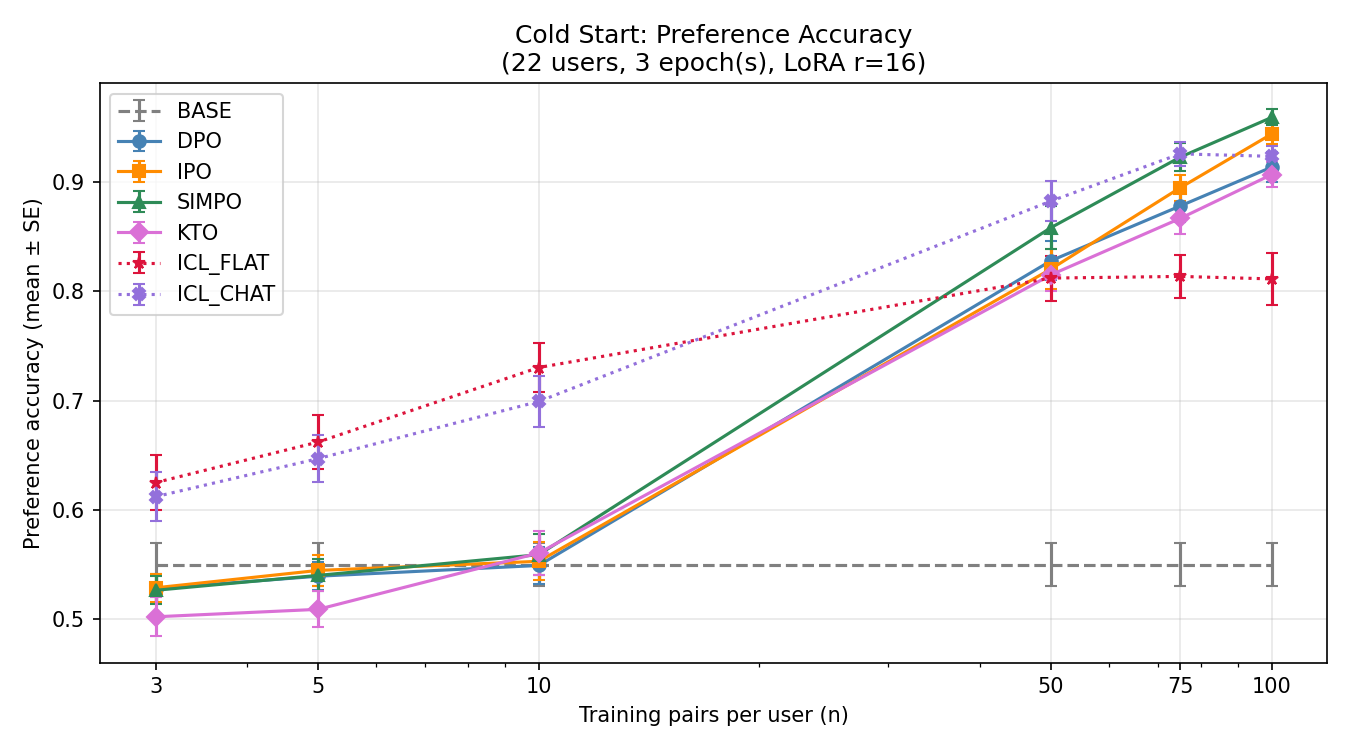
\includegraphics[width=0.48\textwidth]{images/primary_curves_goodreads.png}
\hfill
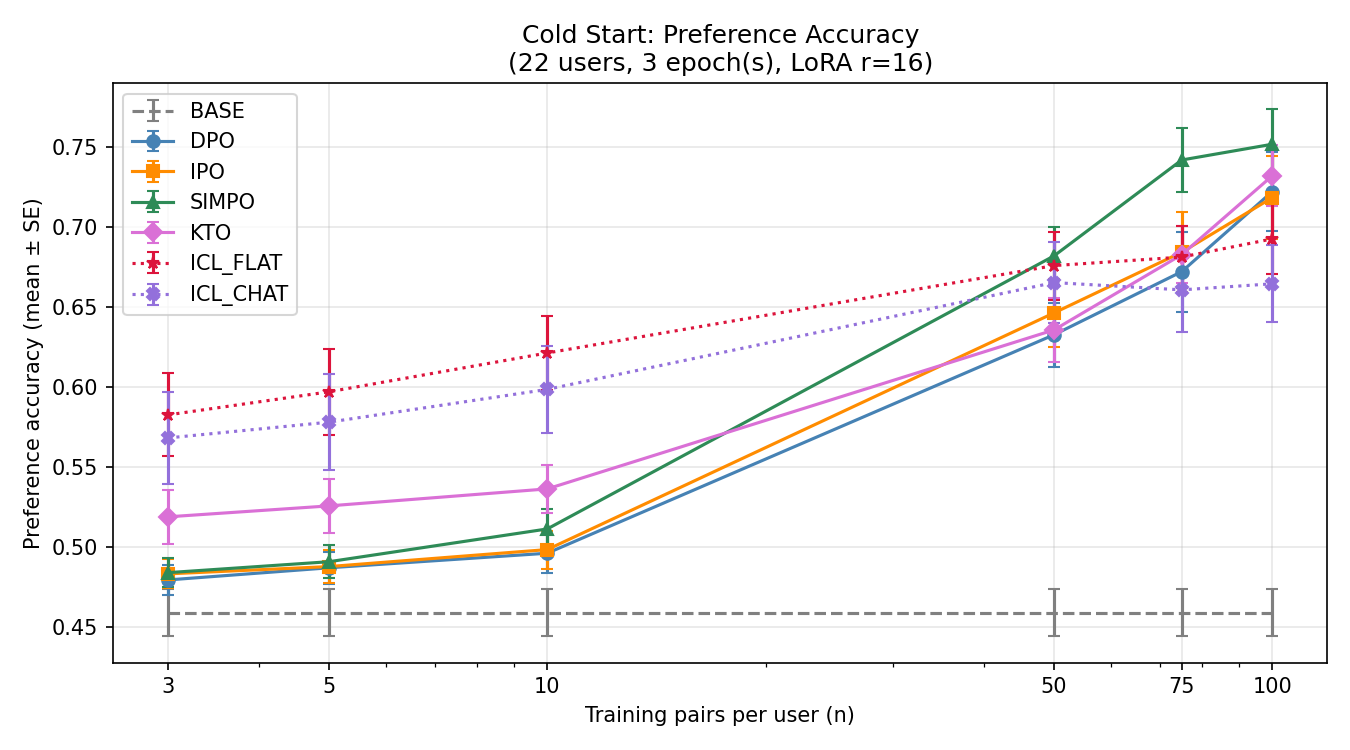
\includegraphics[width=0.48\textwidth]{images/primary_curves_netflix.png}
\caption{Held-out pairwise accuracy by training size $n$ and method. Left: GoodReads. Right: Netflix. Lines are means across users and seeds; shaded regions are $\pm 1$ standard error.}
\label{fig:primary_curves}
\end{figure}

\begin{table}[h]
\centering
\caption{Pairwise accuracy by method and training size. Bold marks the per-column best; $\dagger$ marks significant improvement over the best ICL baseline at the $0.05$ level (paired Wilcoxon at $n = 100$).}
\label{tab:primary_acc}
\begin{tabular}{lcccccc}
\toprule
\textbf{Method} & $n = 3$ & $n = 5$ & $n = 10$ & $n = 50$ & $n = 75$ & $n = 100$ \\
\midrule
\multicolumn{7}{l}{\textit{GoodReads}} \\
base                 & .550 & .550 & .550 & .550 & .550 & .550 \\
dpo                  & .528 & .539 & .549 & .828 & .878 & .914 \\
ipo                  & .529 & .545 & .553 & .820 & .895 & .944 \\
simpo                & .527 & .540 & .559 & .858 & .923 & \textbf{.959}$^\dagger$ \\
kto                  & .502 & .509 & .561 & .815 & .867 & .907 \\
icl\_flat            & \textbf{.625} & \textbf{.662} & \textbf{.730} & .812 & .814 & .811 \\
icl\_chat            & .612 & .647 & .699 & \textbf{.883} & \textbf{.926} & .923 \\
\midrule
\multicolumn{7}{l}{\textit{Netflix}} \\
base                 & .459 & .459 & .459 & .459 & .459 & .459 \\
dpo                  & .480 & .487 & .496 & .633 & .672 & .722 \\
ipo                  & .483 & .488 & .498 & .646 & .684 & .718 \\
simpo                & .484 & .491 & .511 & \textbf{.682} & \textbf{.742} & \textbf{.752}$^\dagger$ \\
kto                  & .519 & .526 & .536 & .636 & .683 & .732 \\
icl\_flat            & \textbf{.583} & \textbf{.597} & \textbf{.621} & .676 & .681 & .692 \\
icl\_chat            & .568 & .578 & .598 & .665 & .661 & .664 \\
\bottomrule
\end{tabular}
\end{table}

The per-user picture matches the means. SimPO wins on $14/22$ users on each dataset, against $7/22$ and $9/22$ for DPO, $10/22$ and $13/22$ for IPO, and $7/22$ and $14/22$ for KTO. The mean ranking and the per-user ranking agree, so the headline is not a few-user artefact.

Two dataset-level differences are worth flagging. The frozen base sits at $0.550$ on GoodReads and at $0.459$ on Netflix, so book titles already carry signal to the pretrained model while movie titles do not. And the ICL baselines swap order across datasets: \texttt{icl\_chat} leads on GoodReads, \texttt{icl\_flat} leads on Netflix. The chat-template advantage is real on books but not on films.

\subsection{Beyond the Cold-Start Cap}

Pushing $n$ from $100$ to $150$ on GoodReads pulls the trained methods toward ceiling and leaves the ICL plateau where it was. Mean accuracy at $n = 150$ is $0.983$ for SimPO, $0.958$ for IPO, $0.932$ for DPO and $0.920$ for KTO, against $0.806$ for \texttt{icl\_flat}. The pairwise ordering established at $n = 100$ in §5.1 is preserved, but the gap between SimPO and the rest of the trained methods narrows as everything approaches the upper bound of the evaluation.

\begin{table}[h]
\centering
\caption{GoodReads pairwise accuracy at $n = 150$, averaged across users and seeds.}
\label{tab:extended_acc}
\begin{tabular}{lc}
\toprule
\textbf{Method} & $n = 150$ \\
\midrule
dpo                 & .932 \\
ipo                 & .958 \\
simpo               & \textbf{.983} \\
kto                 & .920 \\
icl\_flat           & .806 \\
\bottomrule
\end{tabular}
\end{table}

Two notes qualify the comparison with §5.1. The extended sweep was run on a different draw of 22 GoodReads users from the same eligibility pool, with ten users in common with the primary sweep, so the $n = 150$ column is best read as a separate measurement on the same population rather than as a continuation of any individual user's curve. And \texttt{icl\_chat} is not reported here: at $n = 150$ the prompt-side context already exceeds what the chat template can carry under the $8{,}192$-token cap, and the method's accuracy collapses to a level that reflects truncation rather than model behaviour. The \texttt{icl\_flat} variant remains within its working range at this size.

\subsection{Per-User View}

The mean curves in §5.1 hide whether the gain is spread across users or concentrated in a few. Figure~\ref{fig:per_user} shows the full per-user grid: each panel is one user's learning curve under each method, on the same axes as Figure~\ref{fig:primary_curves}. Two facts emerge from the grid that are not visible in the means. No user is harmed by training at $n = 100$: on both datasets, the best trained method beats the frozen base model for every one of the twenty-two users. And no user is left stuck near chance: the worst best-method accuracy is $0.933$ on GoodReads and $0.600$ on Netflix.

\begin{figure}[h]
\centering
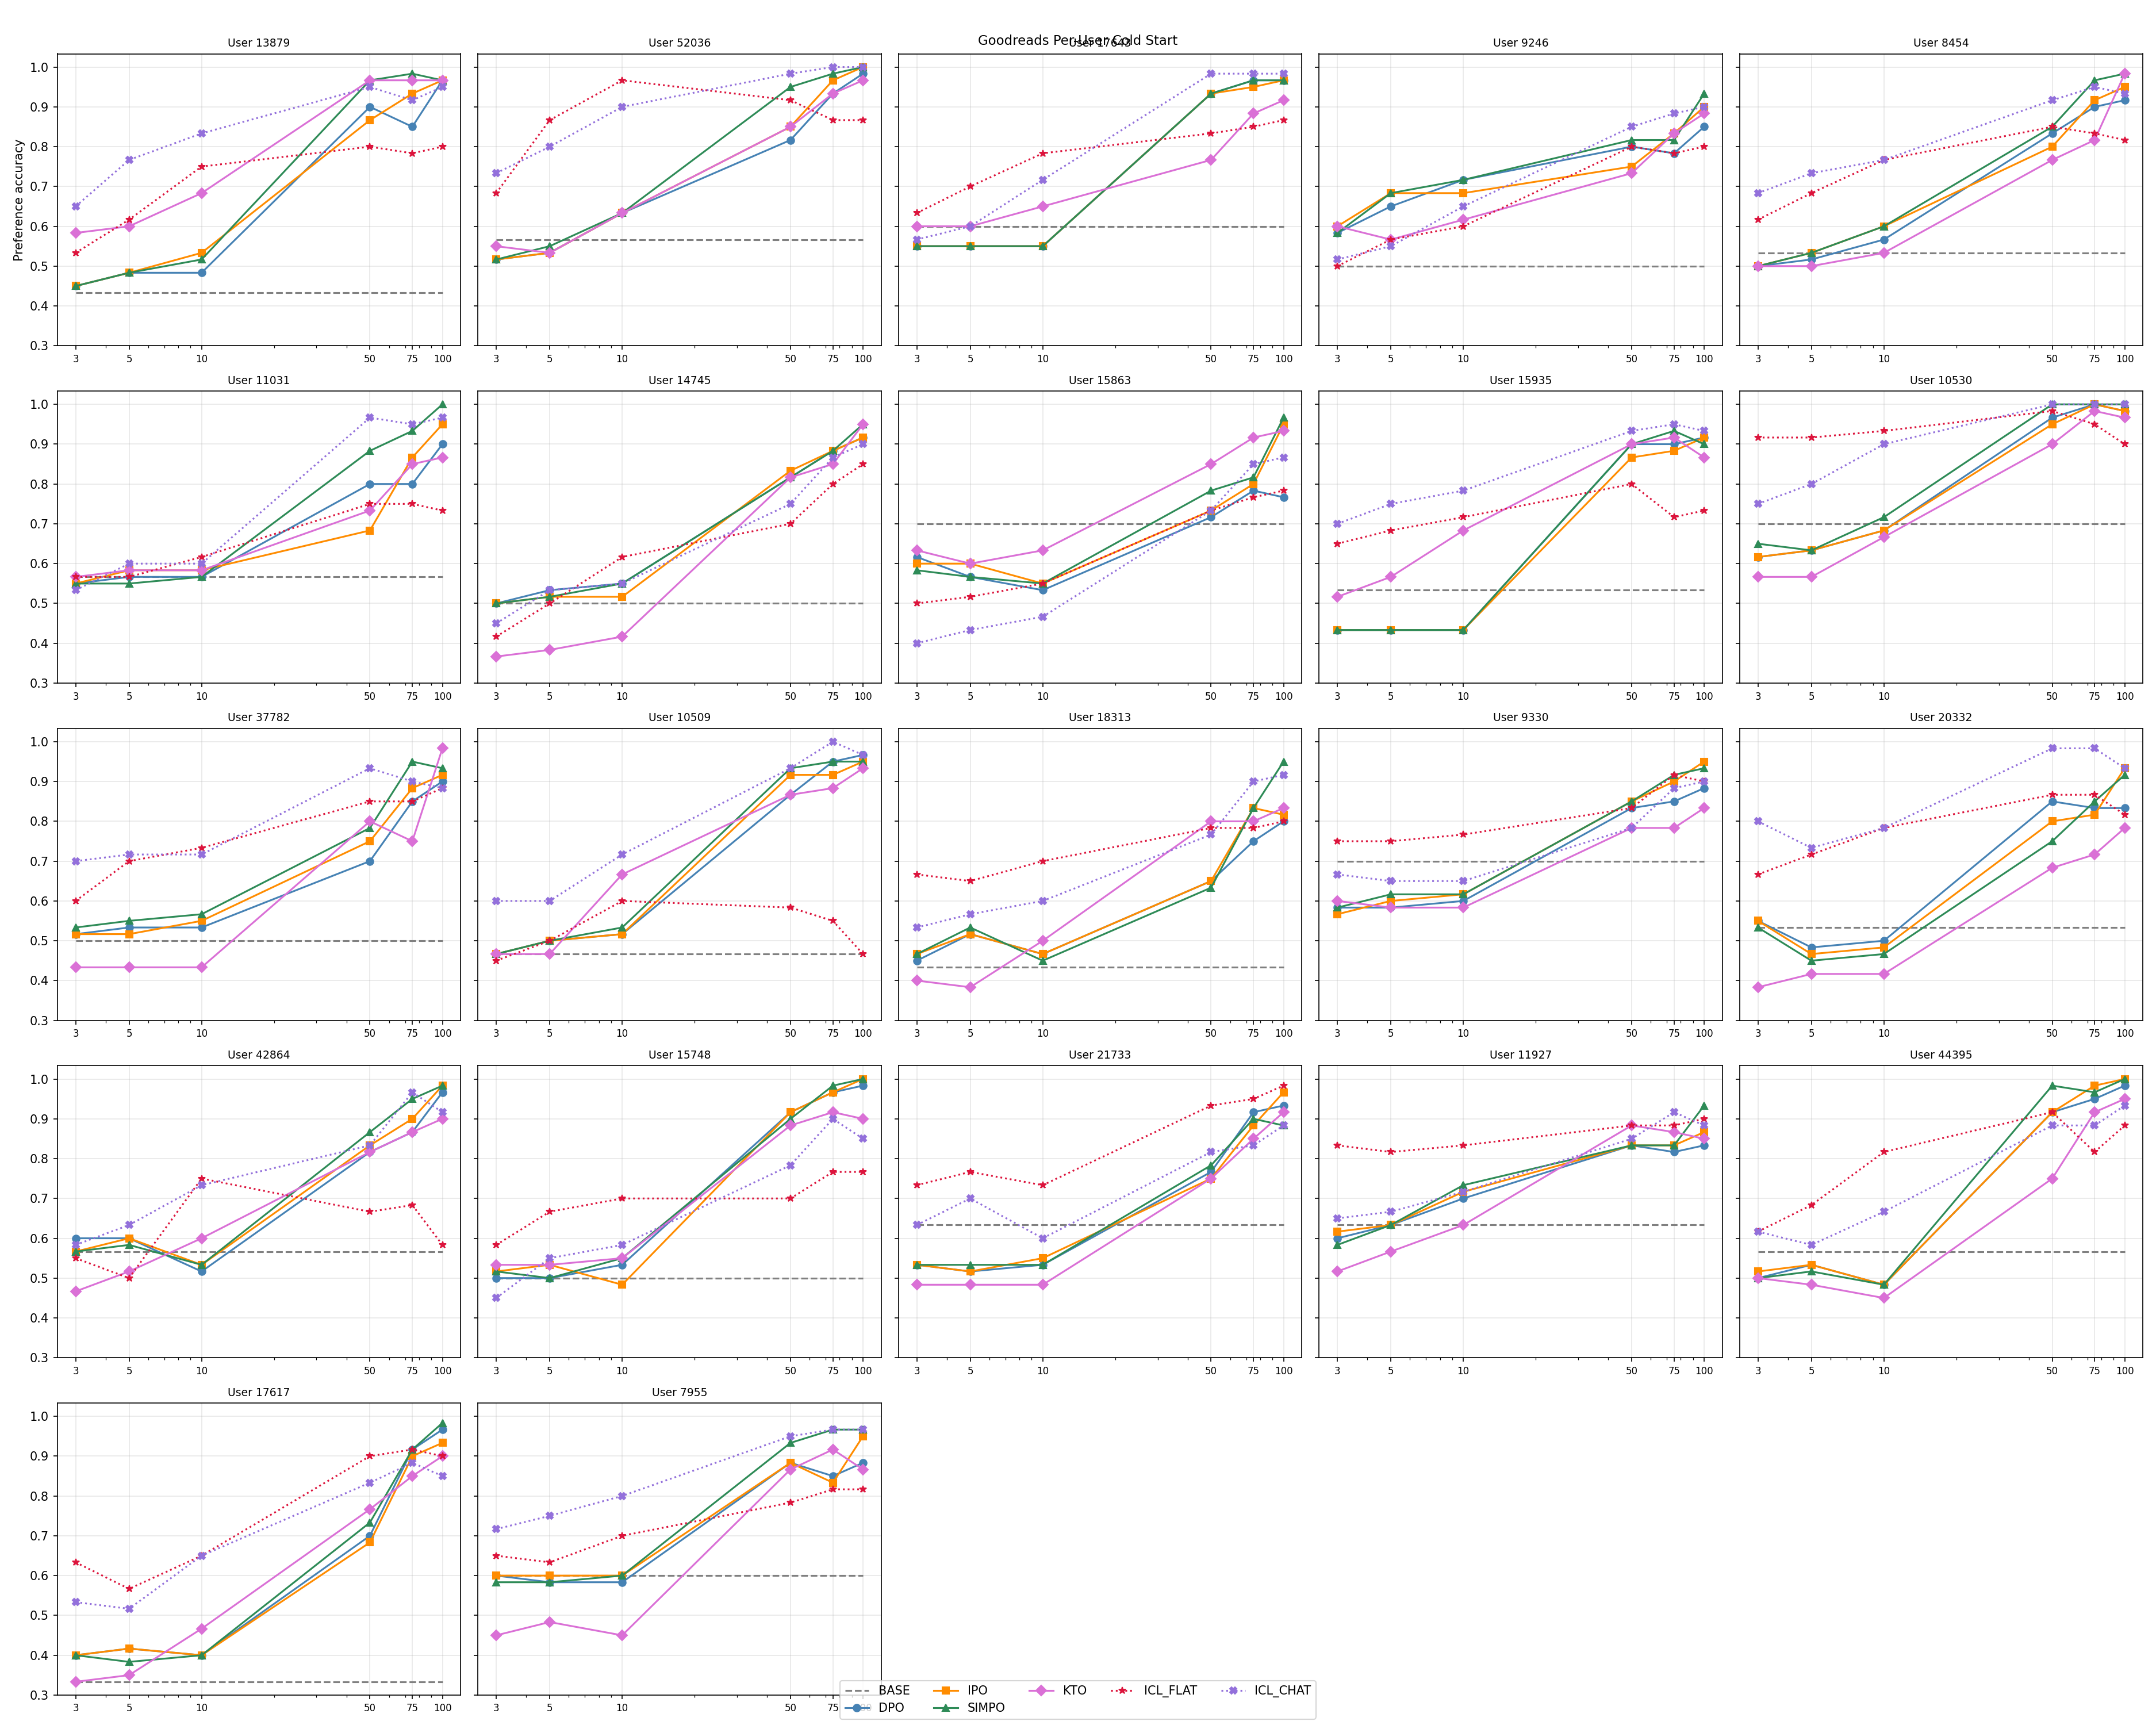
\includegraphics[width=0.48\textwidth]{images/per_user_goodreads.png}
\hfill
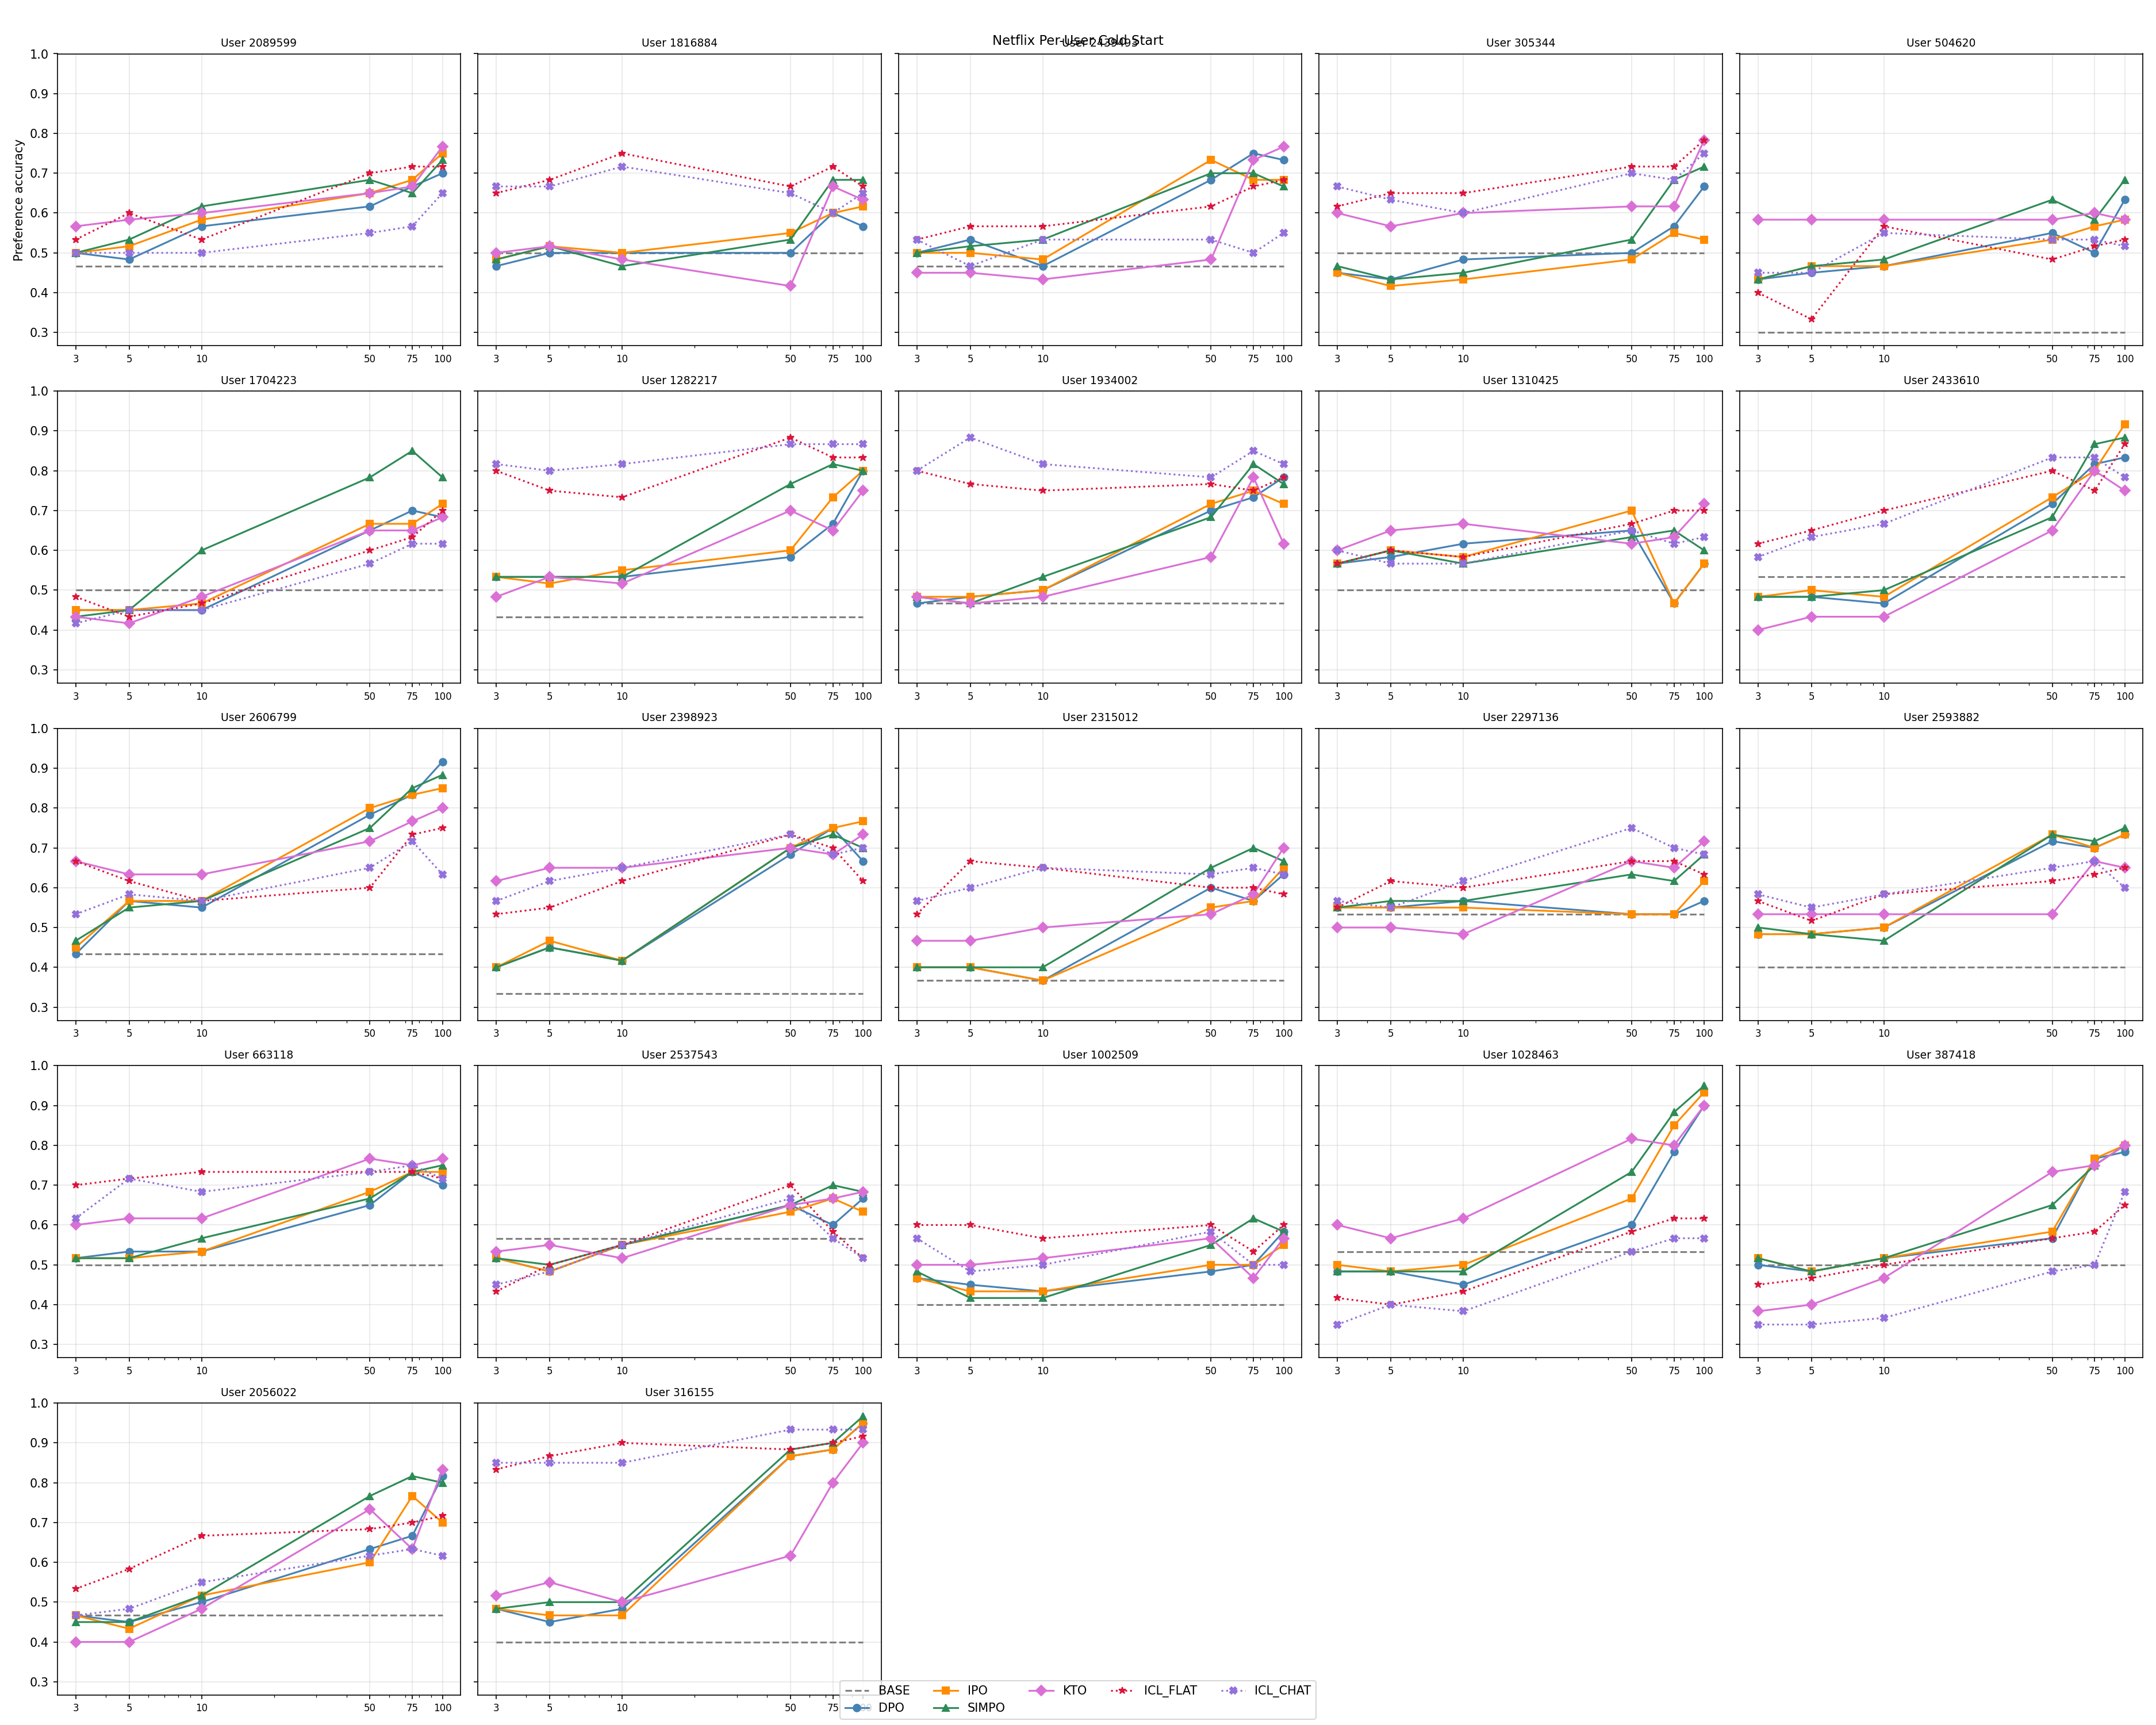
\includegraphics[width=0.48\textwidth]{images/per_user_netflix.png}
\caption{Per-user learning curves on GoodReads (left) and Netflix (right). Each panel is one user; lines are method means across the two seeds.}
\label{fig:per_user}
\end{figure}

\begin{table}[h]
\centering
\caption{Per-user picture at $n = 100$. Columns: spread of the best-method accuracy across the twenty-two users; users for whom no trained method exceeds the base; users where every method stays below $0.60$; outright per-user winner counts among the four trained methods and the two ICL baselines.}
\label{tab:per_user}
\begin{tabular}{lcc}
\toprule
 & \textbf{GoodReads} & \textbf{Netflix} \\
\midrule
Best-method accuracy range          & $[.933,\ 1.000]$ & $[.600,\ .967]$ \\
Users hurt by training              & $0/22$           & $0/22$ \\
Users with no method above $0.60$   & $0/22$           & $0/22$ \\
\midrule
Outright winners (out of $22$) &  & \\
\quad simpo                          & $10$              & $7$ \\
\quad ipo                            & $6$               & $3$ \\
\quad dpo                            & $2$               & $2$ \\
\quad kto                            & $1$               & $7$ \\
\quad \texttt{icl\_chat}             & $2$               & $2$ \\
\quad \texttt{icl\_flat}             & $1$               & $1$ \\
\bottomrule
\end{tabular}
\end{table}

Two things qualify the §5.1 ranking once the per-user picture is in view. SimPO wins the mean comparison and the most users on both datasets, but it is not the per-user winner for $12/22$ GoodReads users and $15/22$ Netflix users --- for those, another trained method matches or exceeds it. The per-user grid also shows that the cold-start advantage of ICL is itself heterogeneous: at $n = 10$, the best ICL baseline beats the best trained method for $20/22$ GoodReads users but only $13/22$ Netflix users. The pattern in the means therefore holds at the user level, but with meaningful per-user variation that any deployment based on these results would need to plan for.
% =============================================================================
% 6. Business Analysis and Decision Framework -- target ~4.5 pp
% THE BA-CORE OF THE THESIS. This is what distinguishes a Business Analytics
% thesis from a generic ML report.
% Three sub-themes:
%   1. Why preference alignment is becoming a strategic capability
%   2. A decision framework for choosing a training method
%   3. The alignment economics that drive the framework
% =============================================================================

\section{Business Analysis and Decision Framework}
\label{sec:business}

\subsection{Market Tendencies}
\label{sec:business:tendencies}

When the first large language models started getting widespread attention, there was a common belief that model performance came mainly from how much data you trained on \citep{brown2020gpt3}. It quickly became apparent that this was not the whole story, and that aligning these models with what users actually wanted was what made them useful in practice. The first widely adopted alignment framework was Reinforcement Learning from Human Feedback, or RLHF, originally proposed by \citet{christiano2017rlhf} for game and robotics environments. The recipe is simple in principle: humans compare pairs of model outputs, a reward model is trained to predict those preferences, and the language model is then optimised against that learned reward. \citet{ouyang2022instructgpt} scaled the recipe to GPT-3 and produced InstructGPT, the direct ancestor of ChatGPT and every aligned LLM that followed. The leap in usefulness was enormous, but the architecture was still one-size-fits-all. A single reward model represented the preferences of a small pool of human annotators, and the resulting policy was shipped to every user as if their tastes matched that pool's.

After this generation of systems reached mass adoption, it became clear that the next step was aligning the model with each individual user. The way the industry has approached this is through context. Instead of retraining the model for every user, you feed it information about who is asking, what they care about, or what task they are trying to do, and let the model condition on that text at inference time. The underlying technique was popularised by Retrieval-Augmented Generation \citep{lewis2020rag} and scaled by follow-up work such as RETRO \citep{borgeaud2022retro}. Productised versions show up everywhere today, from Claude Projects and ChatGPT Memory to Gemini's million-token context window \citep{reid2024gemini}. The appeal is clear: the model keeps all the general world knowledge it learned during pretraining and gets steered toward the task at hand without any weight updates. The important caveat, documented by \citet{liu2023lostmiddle}, is that more context is not always better. Models do not attend uniformly to long prompts, and information buried in the middle of the window is often ignored. This matters for personalisation specifically, because user preferences are exactly the kind of information that piles up over time and risks getting drowned out.

Recommendation systems have always been central to how companies understand their users and connect them with the products they are most likely to want, and for most of their history they have lived behind an interface of ranked lists, grids, and carousels. That interface is now shifting. Users are increasingly comfortable asking for what they want in natural language, and the front door to a product is more and more often a conversation rather than a feed. The academic side has followed quickly. \citet{bao2023tallrec} showed that an LLM can be tuned to act as the recommender itself, \citet{friedman2023recllm} demonstrated this in an explicitly conversational setting, and the survey by \citet{fan2024recllmsurvey} maps how the broader field is reorganising around this transition. The underlying data has not changed, the years of clicks, ratings, and purchases that classical recommenders were built on are still the most valuable signal a company has about its users. What has changed is the surface on which that signal gets used, and the kind of model that needs to consume it.

The findings in this thesis come to inform organisations on how they can tackle these changes and leverage their data, or lack thereof, to enter the LLM world.

\subsection{Business Applications}
\label{sec:business:framework}

These findings become relevant in a business context mainly for companies that use LLMs for customer-facing sales and recommendation, and the natural way to see why is to think about what those companies already have. Almost every consumer business that has been operating for more than a few years sits on a large quantity of discrete user signal, the kind of data classical recommender systems were built to consume. Ratings, watch histories, purchase sequences, thumbs-ups and skips are all the same shape as the preference pairs used throughout this thesis. The work of \citet{bao2023tallrec} and \citet{friedman2023recllm} shows that this signal can be fed into an LLM either by training on it or by placing it in the prompt, and the survey by \citet{fan2024recllmsurvey} confirms this is the direction the field is moving. The question for a company is no longer whether to do it, but how.

That decision is exactly what the results in \cref{sec:results} inform. The crossover between ICL and the trained methods, visible in \cref{fig:primary_curves} and quantified in \cref{tab:primary_acc}, is not just an academic curiosity, it tells a product team where to put a line in their onboarding flow. A music app that hopes a new user will rate ten songs in their first session is operating squarely in the cold-start floor, where ICL leads on both accuracy and cost. A bookseller that nudges every shopper toward fifty ratings before personalising is in the territory where SimPO and IPO have already overtaken the prompt-stuffing baseline. The same business decision, namely how much friction to add to onboarding in exchange for richer personalisation downstream, is also the technical decision of which method to deploy. The two are the same lever seen from two sides.

What makes this practically attractive is that the infrastructure does not change across the regimes. The signal a company needs to collect is the same paired or unpaired preference data either way, and the serving stack only diverges at the last step, with the trained methods loading a small LoRA adapter on top of the same frozen base model that ICL queries directly. \citet{sheng2024slora} showed that thousands of LoRA adapters can be served concurrently on shared infrastructure, which removes the operational objection that per-user training is impractical at scale. The broader point is that the LLM era does not retire the work companies have done on their recommendation stacks over the past decade, it relocates it. The years of clicks and ratings that fed a matrix-factorisation model do not become irrelevant when the front door turns into a chat box, they become the cold-start fuel for whatever personalisation method sits behind that chat box.

\subsection{Alignment Economics}
\label{sec:business:economics}

The decision of whether a company should use in-context learning or shift to a preference-optimisation method is not a one-time architectural choice. It depends on three variables that differ widely between products: how many preferences a user generates during onboarding, how often that same user queries the system afterwards, and how stable their preferences are over time. Mapping the experimental findings from \cref{sec:results} against the cost trajectories documented in the Stanford AI Index 2025 \citep{maslej2025aiindex} lets us turn the abstract trade-off into a decision a product team can actually make.

The empirical anchor is the crossover in \cref{fig:primary_curves}. For $n$ below roughly ten preference pairs, ICL outperforms every trained method on both GoodReads and Netflix, often by a wide margin. Between $n = 10$ and $n = 50$, the trained methods catch up and pass the ICL plateau. At $n = 100$, SimPO leads \texttt{icl\_chat} by 3.6 percentage points on GoodReads and 5.9 points on Netflix, with the gap widening further at $n = 150$. This gives three operational regimes, summarised in \cref{tab:business_regimes}: a cold-start floor where ICL wins on both accuracy and cost, a transition band where the choice is ambiguous, and a steady state where trained methods dominate on accuracy and the question shifts to whether they also win on cost.

\begin{table}[h]
\centering
\caption{Decision regime by training size per user. Recommendations follow directly from the results in \cref{tab:primary_acc} combined with the cost analysis below.}
\label{tab:business_regimes}
\begin{tabular}{lll}
\toprule
\textbf{Regime} & \textbf{$n$ per user} & \textbf{Recommended method} \\
\midrule
Cold-start floor & $n \leq 10$       & ICL \\
Transition band  & $10 < n \leq 50$  & Project engagement before deciding \\
Steady state     & $n > 50$          & SimPO (or IPO with a reference anchor) \\
\bottomrule
\end{tabular}
\end{table}

The Stanford report changes how heavy the cost side of that question is. The cost of running an inference at GPT-3.5 quality dropped from \$20.00 per million tokens in November 2022 to \$0.07 per million tokens by October 2024, a 280-fold reduction in roughly eighteen months \citep{maslej2025aiindex}. Hardware price-performance is improving at 30 percent per year, and a 3.8-billion-parameter Phi-3-mini now matches the MMLU score that a 540-billion-parameter PaLM achieved two years earlier. The practical effect is that the per-query cost of an ICL prompt, which used to be the dominant economic argument against the method, has collapsed. An ICL inference at $n = 100$ carries roughly four thousand extra prompt tokens compared to a trained-model inference. At the Stanford lower bound that adds less than three hundredths of a cent per query. At a more realistic mid-market rate of \$0.20 per million input tokens it is about eight hundredths of a cent. A LoRA training run for one user on a rented A100 costs somewhere between ten and twenty cents, which puts the break-even point at roughly two hundred and fifty queries per user without prompt caching, and around two thousand five hundred queries once prefix caching is in play.\footnote{Anthropic's prompt-caching documentation reports a roughly tenfold cost reduction on cached prefix tokens: \url{https://platform.claude.com/docs/en/build-with-claude/prompt-caching}.}

Two trajectory effects make this picture less stable than \cref{tab:business_regimes} suggests. The first is that ICL economics are improving faster than training economics. \citet{maslej2025aiindex} reports inference cost falling between 9 and 900 times per year depending on the task, while hardware price-performance drops a steadier 30 percent per year. Over the next few cycles, ICL gets cheaper than training does, which pushes the break-even point higher and rewards companies that delay the decision to train. The second is that smaller models are catching larger ones on standard benchmarks, which lifts the floor of base-model capability that ICL exploits. The frozen Llama-3-8B-Instruct used in our experiments is already capable enough to extract signal from book titles at $n = 10$. Two model generations from now, that capability will sit lower on the parameter curve and run faster, which favours ICL further at the entry point.

The recommendation that comes out of this is sequencing rather than choosing. Most consumer products are better off starting with ICL and switching to a trained adapter only for users who cross a clear engagement threshold. The data infrastructure for both is the same, a stream of paired or unpaired preferences accumulated per user. The decision of when to train is then a business question about engagement rather than a technical question about model behaviour, and the empirical crossover in \cref{sec:results} is what tells you where to put the threshold. A company that sees most of its users churn before $n = 10$ should not be training anything. A company that sees its average user generate a hundred preferences a month should be training adapters for everyone past the first session. The Stanford trajectory is what makes this sequenced strategy increasingly attractive, because the cost of getting it wrong in the ICL direction is dropping faster than the cost of getting it wrong in the training direction.

% =============================================================================
% 7. Limitations and Future Work -- target ~1.5 pp
% Be honest. Limitations sections that read as marketing read as defensive.
% =============================================================================

\section{Limitations and Future Work}
\label{sec:limits}

\subsection{Limitations}
\label{sec:limits:lim}

\todo{Be honest about each:

\textbf{Single base model.} Llama-3-8B-Instruct only. Larger and smaller
models may exhibit different sample-efficiency curves; the ranking may not
generalise. Mitigation: report findings as conditional on the base model
and flag this as the most important external-validity threat.

\textbf{Two domains, both well-represented in pretraining.} GoodReads and
Netflix are pop culture, and Llama-3 has demonstrably strong priors on
both. Domains where the LLM has weaker priors -- niche literature,
specialised B2B software, non-English content -- are likely to behave
differently. The familiarity filter (\cref{sec:method:data}) makes this
explicit but doesn't fix it.

\textbf{Preferences derived from explicit ratings.} Real-world preference
data are noisier, sparser, and shaped by survivorship and presentation
effects. The findings here represent an upper bound on what these methods
can achieve.

\textbf{Static, offline setting.} No online adapter updates, no continual
learning, no measurement of how preferences drift over time. All of these
matter operationally and none are addressed here.

\textbf{Compute budget.} Two seeds is enough for direction, not enough
for tight confidence intervals on smaller effect sizes.}

\subsection{Future Work}
\label{sec:limits:future}

\todo{Forward-looking but disciplined:

\textbf{Scale.} Repeat the comparison at $\sim$70B parameters and at smaller
models ($\leq 3$B) deployable on-device. The sample-efficiency curves are
the quantity most likely to change.

\textbf{Domain stress test.} Run the same protocol on a domain where the
base model has thin priors. The familiarity filter would have to be
loosened or replaced.

\textbf{Online and continual alignment.} How does the adapter update as the
user provides more signal over time? Streaming preference learning is a
natural extension of this work.

\textbf{Segment-level adapters.} Per-user adapters do not scale to
millions of users. Clustering users and training one adapter per cluster
is the obvious operationalisation; the question is how much
personalisation quality is lost in the aggregation.

\textbf{Multi-objective alignment.} Real products optimise for preference
fit \emph{and} diversity, safety, and engagement quality. The losses
studied here are single-objective by construction.

\textbf{Cross-domain transfer.} Does aligning on books transfer to films?
The shared latent ``taste'' axis is an open empirical question.}

% =============================================================================
% 8. Conclusion -- target ~1 pp
% No new content. Restate question, headline empirical answer, BA takeaway,
% and one forward sentence.
% =============================================================================

\section{Conclusion}
\label{sec:conclusion}



% ------ References ----------------------------------------------------------
\clearpage
\printbibliography[heading=bibintoc,title={References}]

% ------ Appendices ----------------------------------------------------------
\clearpage
\appendix
% =============================================================================
% Appendix A -- AI Usage Disclosure
% Required by Nova SBE Generative AI guidelines:
%   - AI used to RETRIEVE info: cite as personal communication, in-text
%   - AI used to GENERATE content: name the tool, explain method, date
%   - AI used as EDITING assistance: no disclosure needed
% Source: Nova SBE Guidelines Regarding Usage of Generative AI (current).
% =============================================================================

\section{AI Usage Disclosure}
\label{app:ai}

This appendix discloses the use of generative AI tools during the preparation
of this thesis, following the citation policy and the \emph{Know, Inform,
Assist} principles set out in the Nova SBE Generative AI guidelines
\citep{novasbe-genai}. A clarification is in order before the itemised list.
The thesis studies AI systems and produces AI artefacts: a frozen
Llama-3-8B-Instruct base \citep{llama3}, per-user LoRA adapters
\citep{hu2021lora} trained under DPO, IPO, SimPO and KTO, and the in-context
learning baselines. Those artefacts are the object of study and are documented
in \cref{sec:methodology,sec:design,sec:results}. The present appendix concerns
something different: the AI assistants used \emph{around} that work, as
research, coding and writing aids. Responsibility for every claim, figure and
line of code in the thesis remains solely with the author.

\subsection*{Tools used}

The assistants consulted during the project were Claude Sonnet 4.6, Claude code and Overleaf Writing Assistant.
Access took place between April 6 and May 20.
No paid third-party plug-ins or browsing connectors were used to send any
private or restricted data to these services; see the confidentiality note at
the end of this appendix.

\subsection*{AI used to retrieve information}

The Nova SBE guidelines treat AI as a source of \emph{personal communication}
when it is asked a question and returns an answer that is not independently
recoverable \citep{novasbe-genai}. Used in this way, AI assistants helped
clarify concepts whose primary sources are cited in the body of the thesis.
The main topics on which the assistants were queried are: the mechanics and
relative trade-offs of DPO, IPO, SimPO and KTO
\citep{rafailov2023dpo,azar2024ipo,meng2024simpo,ethayarajh2024kto}, the
geometry and hyper-parameter conventions of LoRA \citep{hu2021lora},
the interpretation of the paired Wilcoxon signed-rank test, and the operational
details of multi-adapter serving \citep{sheng2024slora}. In every case the
authoritative source consulted was the cited publication; the assistant's
output served as a comprehension aid and was discarded once the relevant
passage in the paper was located. Where a factual claim in the thesis rests on
one of these clarifications without an independent secondary source, that
claim was re-verified against the original publication before inclusion. No
in-text \emph{personal communication} citation appears in the body of the
thesis because no claim depends on AI output as a primary source.

\subsection*{AI used to generate content}

Per the Nova SBE guidelines, when AI is used to generate ideas or to develop a
plan, the tool, the method of use and the date of access must be acknowledged
\citep{novasbe-genai}. The following uses fall into this category.

\paragraph{Code and infrastructure.}
Portions of the training and evaluation pipeline were drafted with AI
assistance and then reviewed, executed and modified by the author. This
includes the per-user LoRA training loop, the YAML sweep configurations
referenced in \cref{sec:design}, the KTO row-expansion utility described in
\cref{sec:pair-gen}, the scoring code that groups KTO outputs back into pairs
by \texttt{pair\_id}, and the plotting code used to produce the figures in
\cref{sec:results}. Every code artefact was executed end-to-end on the actual
data.

\paragraph{LaTeX scaffolding.}
The section skeletons, the page-budget comment blocks at the top of each
section, and an initial draft of the \texttt{biblatex} entries in
\texttt{references.bib} were produced with AI assistance. Every bibliographic
entry was then checked against the published source; entries that could not be
verified are flagged in the \texttt{note} field of \texttt{references.bib} and
were either confirmed or removed before submission.

\paragraph{Ideation.} AI assistants were used as a sounding board for the framing of the cold-start problem in \cref{sec:intro}, the structure of the sweep grid in \cref{sec:exp}, and the business-case narrative in \cref{sec:business}. None of the analytical conclusions in those sections was adopted from an assistant's output verbatim: each was either re-derived from the experimental results or supported by a cited source.

\subsection*{AI used in editing assistance}

The Nova SBE guidelines exempt editing assistance from formal acknowledgement
\citep{novasbe-genai}. For transparency, the author notes that AI tools were
used for grammar, clarity and LaTeX-syntax suggestions on prose that the
author had already drafted.

\subsection*{Hallucination and verification}

Generative AI systems can produce confident but inaccurate output, including
fabricated citations \citep{novasbe-genai}. Three concrete safeguards were
applied throughout the project. First, every reference cited in the body of
the thesis was confirmed against the actual publication (DOI or arXiv ID);
items that could not be confirmed are tagged with a \texttt{Verify} note in
\texttt{references.bib} and were resolved before submission. Second, every
piece of AI-assisted code was executed on the real data and its output
compared against expected behaviour described in \cref{sec:methodology}, not
accepted on the strength of the assistant's explanation. Third, numerical
results, statistical tests and figure values reported in \cref{sec:results}
were re-derived from the raw sweep outputs by the author and are
reproducible from the artefacts kept alongside the thesis.

\subsection*{Confidentiality, copyright and data handling}

Both datasets used in this work are publicly released benchmarks: the Netflix
Prize dataset and the GoodReads-10k dataset, as described in
\cref{sec:data}. No personal data, no confidential material from any third
party, no NDA-covered content and no proprietary code base was uploaded to any
external AI service. Where snippets of the author's own code or LaTeX were
shared with AI assistants for editing assistance, the content involved no
material under embargo and no identifying information about the dataset
subjects.

\subsection*{Accountability}

In line with the Nova SBE guidelines, the responsibility to discuss, defend
and justify the merit and sources of the content of this thesis rests solely
with the author \citep{novasbe-genai}. Every methodological choice, every
analytical step and every conclusion reported in the body of the document can
be re-derived from the materials cited and reproduced from the artefacts kept
alongside the submission. The use of AI tools described above accelerated
drafting and verification; it did not substitute for the underlying decisions,
which remain the author's own.

\end{document}